\chapter{CAPTCHAs}\label{cap:captchas}

Neste capítulo abordaremos como funcionam os principais tipos de CAPTCHA conhecidos. Daremos um enfoque especial aos CAPTCHAs baseados em texto, objeto de estudo do presente trabalho. Na secção \ref{sec:captchatexto} daremos uma definição mais precisa para este HIP em particular.

\section{CAPTCHAs}\label{sec:captchas}

CAPTCHAs \cite{captcha2003} ou HIP \cite{lectures2005HIP}, são um conjunto de técnicas que tem como objetivo discernir a ação automatizada de robôs da ação de seres humanos na Rede Mundial de Computadores. Esses filtros tem sido usados de forma efetiva na defesa de diversos tipos de ataque: proteger informações sensíveis, como \textit{e-mail} e dados pessoais; impedir tentativas de \textit{login} automatizados; coibir acesso massivo à sistemas de bases de dados; entre outros. Entretanto, desde as primeiras aplicações até os dias de hoje, existe uma corrida co-evolucionária entre atacantes e defensores. Por um lado, algoritmos de '\textit{quebra}' de CAPTCHA se  tornam cada vez mais sofisticados e precisos. Por outro lado, filtros mais complexos são desenvolvidos. Contudo, como explicado por Chellapilla \textit{Et al.} \cite{lectures2005HIP}, existe um balanço entre complexidade e factibilidade que os defensores devem buscar, explorando habilidades em que humanos ainda não foram ultrapassados por máquinas. O autor também estima que os requisitos mínimos de um HIP para ser considerado efetivo é ser solúvel por humanos $90\%$ das vezes e é considerado '\textit{quebrado}' se puder ser enganado por robôs em mais do que $1\%$ das tentativas, sendo esses valores dependentes do custo de repetição do ataque.

De forma geral, esses filtros podem ser formulados como um desafio sobre um conjunto de domínio cuja a resposta é um token. O domínio pode ser um trecho de áudio, uma sequencia de imagens ou até mesmo o histórico de navegação do desafiado. O token pode ser constituído de um conjunto de ações, o texto extraído de um áudio ou imagem, ou possuir um histórico de navegação confiável. Podem ainda ser constituídos de uma única etapa ou de varias. Uma categorização dos tipos de CAPTCHA pode ser encontrado em \cite{singh2014survey}. Na figura \ref{diffcaptchas} podemos ver diferentes tipos de CAPTCHAs gerados com a biblioteca de código aberto \textit{Securimage} \cite{securimage}.

\begin{figure}[ht]
	\caption{Diferentes tipos de CAPTCHAs}
	\label{diffcaptchas}
	\begin{subfigure}{.5\textwidth}
		\centering
		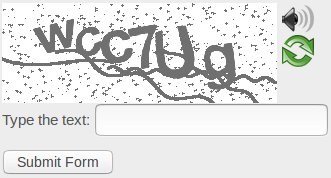
\includegraphics[width=.9\linewidth]{figuras/captcha_letras.png}
		\caption{Letras}
	\end{subfigure}
	\begin{subfigure}{.5\textwidth}
		\centering
		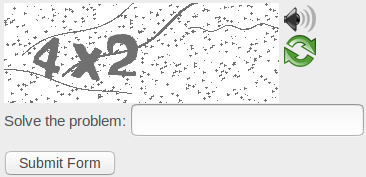
\includegraphics[width=.9\linewidth]{figuras/captcha_mat.png}
		\caption{Desafio matemático}
	\end{subfigure}%
	\vspace{.05\linewidth}
	\begin{subfigure}{.5\textwidth}
		\centering
		
\includegraphics[width=.9\linewidth]{figuras/captcha_texto.png}
		\caption{Duas palavras}
	\end{subfigure}
	\begin{subfigure}{.5\textwidth}
		\centering
		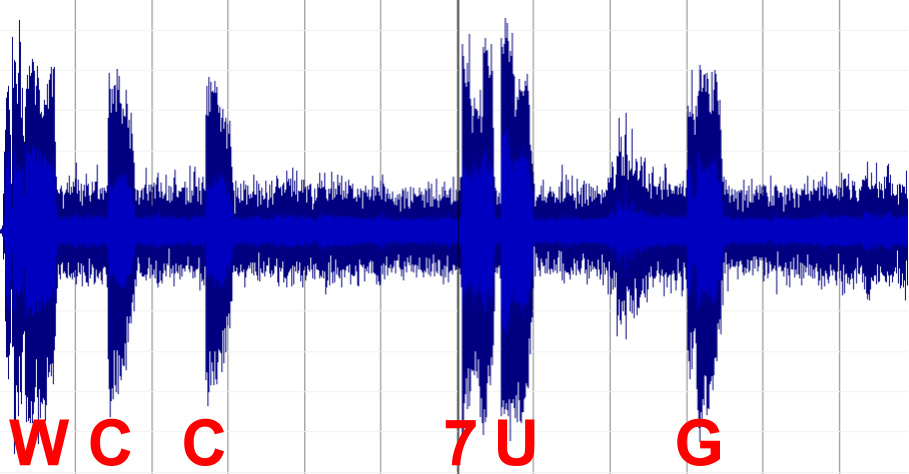
\includegraphics[width=.9\linewidth]{figuras/captcha_audio2.png}
		\caption{Áudio}
	\end{subfigure}
	\small (a) O desafiado deve reconhecer corretamente um texto formado por caracteres não correlacionados. (b) O desafio consiste em extrair e resolver corretamente um problema simples de álgebra. (c) Identificar palavras sorteadas de um repositório. (d) O desafio consiste com extrair corretamente um conjunto de símbolos codificados em áudio. Todos os exemplos foram gerados pelo autor utilizando a biblioteca Securimage. O espectro de intensidades em (d) foi gerado pelo autor a partir do áudio de um CAPTCHA gerado pela biblioteca.
\end{figure}

O processo de '\textit{quebra}' envolve duas ideias principais: explorar vulnerabilidades e/ou uso de algoritmos inteligentes. Por serem testes automatizados, CAPTCHAs geralmente apresentam algum padrão de comportamento ou falha de projeto. A padronização na geração de desafios pode permitir que um atacante desenvolva heurísticas de ataque. Imagens com mesmo espaçamento de caracteres ou padrões repetitivos podem ser explorados e facilitar a segmentação da imagem, como foi explorado por \cite{naivecaptcha}. Falhas ou vieses no projeto desses métodos também podem expor brechas. Quanto ao uso de algoritmos inteligentes, redes neurais recebem um lugar de destaque devido a flexibilidade e capacidade de generalização que esses modelos conseguem alcançar. O uso dessa classe de algoritmos foi a abordagem escolhida por \cite{captcha_break_2013} e \cite{lectures2005HIP}, por exemplo. Redes neurais são exploradas no capítulo \ref{cap:neurais}.

Ao longo dos anos os domínio e os desafios tem evoluído em complexidade, na medida que os atacantes evoluem em técnicas de ataque. Um exemplo da co-evolução desses sistemas é a forma como o sistema reCaptcha \cite{recaptcha1} tem mudado ao longo dos anos. Quando proposto, o sistema era baseado em trechos de livros e jornais antigos em que os melhores algoritmos conhecidos à época falharam em uma tarefa de OCR (do inglês optical character recognition). Trechos que não haviam sido corretamente identificados (teste) eram separados e exibidos para humanos juntamente com imagens de trechos onde o reconhecimento havia falhado (controle). Teste e controle eram comparados para certificar a atuação humana. Quando proposto, os autores alegaram que humanos seriam capazes de resolver o desafio em quase todos os casos e que comutadores teriam chance quase nula de passarem desapercebidos, já que o repositório de exemplos era composta por imagens em que as técnicas vigentes à época haviam falhado. Porém, poucos anos depois, avanços em técnicas de OCR baseadas em redes neurais obtiveram $99\%$ de precisão na base de palavras utilizada por esse sistema \cite{captcha_break_2013}, inviabilizando o uso dessa técnica e forçando o reCaptcha a evoluir para uma segunda versão. Nessa nova abordagem, os dados de navegação dos usuários são analisados por um algoritmo de risco. Caso uma pontuação mínima seja atingida, o usuário é considerado humano, caso contrário, é exposto a problemas conhecidamente difíceis para computadores, como reconhecimento de objetos, contextualização de imagens e busca de similaridades, combinados com diferentes ações que devem ser performadas pelo usuário. Entretanto, Sivakorn \textit{Et al.} \cite{imarobot} mostraram que explorando-se os critérios de avaliação de risco, seria possível enganar o sistema em $85\%$ das vezes, forçando a constante atualização dos desafios.

\section{Captchas de texto}\label{sec:captchatexto}

Nos CAPTCHAs baseados em texto, uma imagem contendo uma sequência de caracteres é exibida ao desafiado. O teste consiste em conseguir recuperar corretamente o texto codificado na imagem. Matematicamente, uma imagem com altura $A$, largura $L$ e $C$ canais pode ser representada como um tensor $\mathbf{X} \in \Re^{A,L,C}[0,1]$, de modo que  $X_{ijk}$ representa a intensidade do pixel na posição $(i,j)$ canal $k$. Um token é uma sequencia $u$ sob um alfabeto de símbolos $\Sigma$, podendo o comprimento da sequência ser limitado ou não. Assim, '\textit{quebrar}' um CAPTCHA de texo é encontrar um mapa $f(\mathbf{X}) \rightarrow u$ que obtenha uma taxa de acerto maior do que $1\%$ como comentado na seção \ref{sec:captchas}. Um sistema de CAPTCHA torna-se completamente inútil se não conseguir diferenciar humanos de robores.

Quanto à imagem, usualmente são utilizadas adição de ruído, linhas e/ou grades para dificultar o processo de segmentação de caracteres, bem como efeitos de distorção, corrosão e/ou dilatação, e transformações geométricas como rotação e translação, entre outros. Em desafios mais simplórios, o número de canais pode ser reduzido, podendo a imagem ser representada como em tons de cinza. Em desafios mais complexos, o espaços de canais é explorado, aumentando algebricamente as possibilidades representação, mantendo, todavia, a factibilidade do desafio para seres humanos, dada nossa facilidade em distinguir cores\footnote{Nem sempre esta afirmação é verdadeira. De fato, pessoas que sofrem da Síndrome de Dalton, o Daltoninsmo, podem ter dificuldades em resolver desafios que explorem diferentes cores. O balanço entre complexidade e inclusão de pessoas com necessidades especiais ainda é uma questão em aberto no projeto de CAPTCHAs.}. É possível explorar imagens sintéticas, geradas de forma automatizada por computadores, ou imagens naturais, como paisagens ou textos em fotos reais. 

Quanto ao texto, diferentes complexidades podem ser adicionadas. Fixadas as demais variáveis, a dificuldade do desafio é usualmente proporcional ao tamanho de alfabeto escolhido. Dentre os mais simples, o conjunto dos números $\Sigma = {0123456789}$ possui apenas dez símbolos. No outro extremo, os logogramas chineses constituem alfabetos com um número indeterminado de símbolos, com as representações mais usuais se limitando a algo em torno de $3000$ caracteres. A tipografia também interfere na dificuldade de resolver um CAPTCHA. Para o mesmo alfabeto $\Sigma$ existem diferentes possibilidades de representação gráfica dos seus caracteres. Fontes regulares tendem a fornecer representações mais simples, com a desvantagem de serem facilmente reconhecíveis por OCR. No outro extremo, fontes simbólicas e caracteres escritos à mão podem representar um grande desafio para máquinas. Quando os símbolos são sorteados de forma aleatória, humanos e máquinas, tipicamente, presenciam maiores dificuldades, dado que cada entrada deve ser reconhecida separadamente (errar o reconhecimento um símbolo significa uma falha completa). Quando sorteamos palavras a partir de um repositório, o desafio se torna mais amigável para humanos, primeiro por termos uma facilidade maior em reconhecer padrões do que especifidades e segundo por nos permitir o uso indireto de outras fontes de conhecimento para a solução do problema. Se soubermos que os textos estão em Português, por exemplo, podemos esperar que nenhuma palavra conterá uma subsequência \textit{tt} (gramaticalmente incorreto) ou que uma vogal será, provavelmente, seguida por uma consoante ou por uma vogal diferente (padrão mais frequente na língua). Entretanto, quando o repositório de palavras é exposto, atacantes podem desenvolver heurísticas para explorar o problema, como um dicionário de palavras ou correção gramatical para aprimorar a eficiência das técnicas. Além disso, repositórios de palavras induzem correlações entre os caracteres, o que limita bastante o espaço de possíveis tokens. Ver \cite{bursztein2011text} para um apanhado de CAPTCHAs de texto utilizados pelo mundo e \cite{captcha_review_2017} para uma a evolução desses sistemas ao longo dos anos. Na figura \ref{captchasbrasil} temos alguns exemplos utilizados por instituições brasileiras.

\begin{figure}[ht]
	\caption{Diferentes CPATCHAs de texto em uso por instituições brasileiras.}
	\label{captchasbrasil}
	\begin{subfigure}[t]{.475\textwidth}
		\centering
		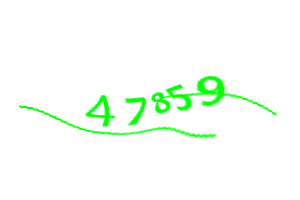
\includegraphics[width=.9\linewidth, height=.4\linewidth]{figuras/captcha_banco_central.png}
		\caption{Banco Central do Brasil}
	\end{subfigure}
	\hspace{.05\textwidth}
	\begin{subfigure}[t]{.475\textwidth}
		\centering
		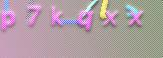
\includegraphics[width=.9\linewidth, height=.4\linewidth]{figuras/captcha_inss.jpeg}
		\caption{Instituto Nacional do Seguro Social (INSS)}
	\end{subfigure}%
	
	\vspace{.05\linewidth}
	\begin{subfigure}[t]{.475\textwidth}
		\centering
		
\includegraphics[width=.9\linewidth, height=.4\linewidth]{figuras/captcha_itau.jpeg}
		\caption{Banco Itaú}
	\end{subfigure}
	\hspace{.05\textwidth}
	\begin{subfigure}[t]{.475\textwidth}
		\centering
		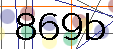
\includegraphics[width=.9\linewidth, height=.4\linewidth]{figuras/captcha_mec.png}
		\caption{ Ministério da Educação (MEC)}
	\end{subfigure}%
	
	\vspace{.05\linewidth}
	\begin{subfigure}[t]{.475\textwidth}
		\centering
		
\includegraphics[width=.9\linewidth, height=.4\linewidth]{figuras/captcha_mprj.jpeg}
		\caption{Ministério Público do Estado do Rio de Janeiro (MPRJ)}
	\end{subfigure}
	\hspace{.05\textwidth}
	\begin{subfigure}[t]{.475\textwidth}
		\centering
		
\includegraphics[width=.9\linewidth, height=.4\linewidth]{figuras/captcha_tjpe.png}
		\caption{Tribunal de Justiça do Estado de Pernambuco (TJPE)}
	\end{subfigure}%
	\vspace{.05\linewidth}	
	\small 
	(a) Disponível em: \url{https://www3.bcb.gov.br/faleconosco/#/login/consultar}. Acesso em: 23/06/201.
	(b) Disponível em: \url{https://cadsenha.inss.gov.br/cadsenha-internet-web/faces/pages/segurado/entradaNitNb.xhtml}. Acesso em: 23/06/201. 
	(c) Disponível em: \url{https://bankline.itau.com.br/boletos-novosite/simulador_etapas_boletos_02.htm}. Acesso em: 23/06/201.
	(d) Disponível em: \url{http://painel.mec.gov.br/painel/captcha}. Acesso em: 23/06/201. 
	(e) Disponível em: \url{http://www.mprj.mp.br/comunicacao/ouvidoria/consulte-a-sua-comunicacao}. Acesso em: 23/06/201. 
	(f) Disponível em: \url{https://srv01.tjpe.jus.br/consultaprocessualunificada/}. Acesso em: 23/06/201.
\end{figure}

